\documentclass[reprint,aps,prl,twocolumn,nofootinbib,longbibliography]{revtex4-2}

\usepackage[T1]{fontenc}
\usepackage{lmodern}
\usepackage{microtype}
\usepackage{amsmath,amssymb,amsthm,mathtools}
\usepackage{bm}
\usepackage{siunitx}
\usepackage{xcolor}
\usepackage{booktabs}
\usepackage{graphicx}
\usepackage{tikz}
\usepackage{pgfplots}
\pgfplotsset{compat=1.18}
\usepackage[hidelinks]{hyperref}

% --- Macros ---
\DeclareRobustCommand{\Sel}{\mathrm{Sel}}
\DeclareRobustCommand{\CL}{\mathrm{CL}}
\DeclareRobustCommand{\Budget}{\mathbf{B}}
\DeclareRobustCommand{\Lam}{\bm{\Lambda}}
\DeclareRobustCommand{\Bth}{B_{\mathrm{th}}}
\DeclareRobustCommand{\Bcx}{B_{\mathrm{cx}}}
\DeclareRobustCommand{\Bleak}{B_{\mathrm{leak}}}
\DeclareRobustCommand{\Nlocal}{\mathsf{N}_{\mathrm{Local}}}
\DeclareRobustCommand{\Ncosmic}{\mathsf{N}_{\mathrm{Cosmic}}}
\DeclareRobustCommand{\TDS}{\ensuremath{T_{\mathrm{D6}}}}
\DeclareRobustCommand{\Dsix}{\ensuremath{D_{6}}}
\DeclareRobustCommand{\AoE}{AoE}
\DeclareRobustCommand{\eps}{\varepsilon}
\DeclareRobustCommand{\Lmax}{\ell_{\max}}
\DeclareRobustCommand{\ethop}{\eth}
\DeclareRobustCommand{\Eul}{\mathrm{Eul}}
\newcommand{\ThreeJ}[6]{\begin{pmatrix} #1 & #2 & #3 \\ #4 & #5 & #6 \end{pmatrix}}
\providecommand{\eth}{\text{\dh}}

\begin{document}

\title{Geometric Impedance in the CMB: Low-\texorpdfstring{$\ell$}{l} Alignments and the Hubble Tension from a $D_6$ Observer Scaffold (Audit-First v2)}

\author{Vladimir Ilinov}
\affiliation{Independent Researcher}
\date{\today}

\begin{abstract}
We revisit two long‑standing large‑angle puzzles in the CMB—the quadrupole–octupole alignment (the “Axis of Evil”) and the \(\sim\!8\%\) Hubble tension—using a simple, observer‑geometry model. The only assumption is a very weak, direction‑dependent weighting of the sky with a six‑fold (D6) symmetry, multiplying an otherwise isotropic CMB map. This minimal modulation makes three concrete predictions on Planck 2018 temperature data. First, the quadrupole and octupole share a common axis that matches the D6 geometry: the alignment rejects isotropy in our Monte Carlo (no exceedances) and the D6 fit is significant (\(p{=}0.015\)) with the expected orientation. Second, the fractional \(H_0\) offset inferred locally versus from the CMB is predicted without tuning at \(0.082865\), matching the observed \(0.083086\) (\(0.27\%\) difference). Third, the hemispherical power asymmetry aligns with the D6 axis (\(p{=}0.008\), \(\approx\!10^\circ\) offset). Two cross‑checks are null, as expected for a weak modulation: a D6‑aware bispectrum test (\(p\!\approx\!0.23\)) and a cold‑spot alignment test (\(p\!\approx\!0.20\)). All results are fully auditable in the repository (code, inputs, run logs, and figures). The data support a simple geometric, observer‑dependent explanation for the large‑angle features, without introducing new early‑Universe parameters.
\end{abstract}

\maketitle

\section{Introduction}
Two persistent large-angle anomalies have resisted standard explanations: (i) the alignment of the CMB quadrupole and octupole (the AoE) and (ii) the $\sim\!8\%$ discrepancy between local and CMB-inferred $H_0$. We show both follow from \emph{observer geometry}: in CT, the observer is a structured pattern (P8), a finite $D_6$-symmetric contact graph \TDS\ selected at the local equilibrium (Selected Equalization Point, SEP). Observation through this lens induces a \emph{geometric impedance} $Z_{D_6}(\hat{n})$ that modulates an intrinsically isotropic background, imprinting $D_6$ symmetry at the largest angular scales and predicting an $H_0$ calibration offset from the hierarchical gradient between $\Nlocal$ and $\Ncosmic$.

\section{From null defect search to impedance}
We first pursued CT-predicted synchronization mosaics via a gauge-invariant wavelet-phase-coherence (WPC) pipeline on Planck maps. After multi-frequency gating, half-mission consistency, and a mandatory \emph{resolution-dependence} falsifier, leading candidates failed publication-grade thresholds (Table~\ref{tab:wpc}). This null outcome, together with CT locality and gauge/Ad-invariance, motivated a pivot: the CMB is the equilibrium scaffold of the cosmic phase, and the act of observation through \TDS\ induces anisotropy (\emph{geometric impedance}).

\section{Theory: selection, budgets, and impedance}
\paragraph{Selection principle and budgets.}
In CT a pattern $A$ persists iff
\begin{equation}
\Sel_{\Lam}(A) = \CL(A)-\langle \Lam, \Budget(A)\rangle \ge 0\,,\label{eq:Sel}
\end{equation}
with budgets from a Hodge decomposition on the contact graph, $\Budget=(\Bth,\Bcx,\Bleak)$. At SEP, multipliers $\Lam$ fix the local physics; the canonical $D_6$-symmetric tile \TDS\ realizes the minimal scaffold.

\paragraph{Geometric impedance.}
Let $I_{\mathrm{CMB}}$ be the intrinsic, isotropic background and $I_{\mathrm{obs}}$ the measured sky. Observation through \TDS\ yields
\begin{equation}
I_{\mathrm{obs}}(\hat{n}) = Z_{D_6}(\hat{n})\, I_{\mathrm{CMB}}(\hat{n})\,,\label{eq:obs}
\end{equation}
with a minimal $D_6$-invariant form
\begin{equation}
Z_{D_6}(\hat{n}) = Z_0 + \eps\,\sum_{A\in \mathrm{Axes}(D_6)} w_A\, (\hat{n}\!\cdot\! \bm{A})^2\,,\label{eq:Z}
\end{equation}
where $\{\bm{A}\}$ are the primary and in-plane axes. Expanding $Z_{D_6}(\hat{n})=\sum_{LM}z_{LM} Y_{LM}(\hat{n})$, the observed multipoles are linearly coupled via Gaunt coefficients:
\begin{align}
a_{\ell m}^{\mathrm{obs}} &= \sum_{\ell' m'} K_{\ell m}^{\ell' m'}\, a_{\ell' m'}^{\mathrm{cmb}},\label{eq:coupling}\\[2pt]
K_{\ell m}^{\ell' m'} &= \sum_{LM} z_{LM}\, (-1)^m\, \sqrt{\frac{(2\ell{+}1)(2\ell'{+}1)(2L{+}1)}{4\pi}} 
\nonumber\\[-2pt]
&\quad \times \ThreeJ{\ell}{\ell'}{L}{0}{0}{0}
\nonumber\\[-2pt]
&\quad \times \ThreeJ{\ell}{\ell'}{L}{-m}{m'}{M}.
\nonumber
\end{align}
$D_6$ symmetry imposes selection rules (Appendix~\ref{app:selection-rules}), maximizing effects at low $\ell$.

\paragraph{Two key predictions.}
(i) \textbf{P-T2 (AoE)}: the preferred axes of $\ell{=}2,3$ align with the $D_6$ primary axis, in the canonical orientation of \TDS\ (up to sky rotation). (ii) \textbf{P-H2 (Hubble tension)}: a parameter-free hierarchical calibration gradient between $\Nlocal$ and $\Ncosmic$ implies a fixed fractional offset $\Delta H_0/H_0$ computable from the independently calibrated \TDS\ energetic ratio.

\section{Data and pipeline}
\textbf{Inputs.} Planck SMICA map: \url{data/raw/planck/COM_CMB_IQU-smica_2048_R3.00_full.fits}. Hubble JSONs: \url{data/raw/local_universe/h0_local.json}, \url{data/raw/planck/planck_h0_cosmic.json}. CT params: \url{data/raw/ct_params/t_d6_parameters.json}. All reported numbers are read from the run directories cited below.

\textbf{Statistics.} Low-$\ell$ axes from multipole maps; AoE statistic $\mathcal{A}_{23}=|\hat{\bm v}_2\cdot\hat{\bm v}_3|$. Significances via Monte Carlo (isotropic Gaussian skies and random-$D_6$ orientation nulls). Hemispherical asymmetry from hemispheric power contrast along the $D_6$ axis. Bispectrum tests via equilateral proxy and an anisotropic $m$-selection statistic.

\section{Results}
\paragraph{Axis of Evil (P-T2).} We find $\mathcal{A}_{23}=0.999674$ with best $D_6$ score $0.999919$ at Euler $\Eul_{zyz}=(0,\,8.815\times10^{-9},\,0)$; $p_{D_6}=0.015$ with zero isotropic exceedances in the reported run (\url{results/runs/20251023_143945_pt2_alignment}). Figure~\ref{fig:aoe-corrected} shows the observed axes and the $D_6$ primary.

\paragraph{Hemispherical asymmetry.} Along the $D_6$ axis we obtain $A_{D_6}=-0.0573$ with $p=0.008$ and best-axis offset $\SI{10.3}{\degree}$ to $D_6$ (\texttt{results/runs/20251024\_074842\_hemispherical\_asymmetry}).

\paragraph{Hubble tension (P-H2).} Observed fractional tension $0.083086$ vs CT prediction $0.082865$ (parameter-free) agree to $0.27\%$ (\texttt{results/runs/20251024\_074832\_ph2\_hubble}).

\paragraph{Bispectrum and cold spot.} The $D_6$-anisotropic bispectrum yields $p=0.228$ with $S_{\mathrm{obs}}=5.165\times 10^{-15}$ (\texttt{results/runs/20251023\_181524\_pt1\_d6\_anisotropic}). The global projection run gives $p\approx 0.51$ (\texttt{results/runs/20251024\_144608\_pt1\_bispectrum}). Cold spot–axis alignment is null with $p\approx 0.195$.

\begin{figure*}[t]
  \centering
  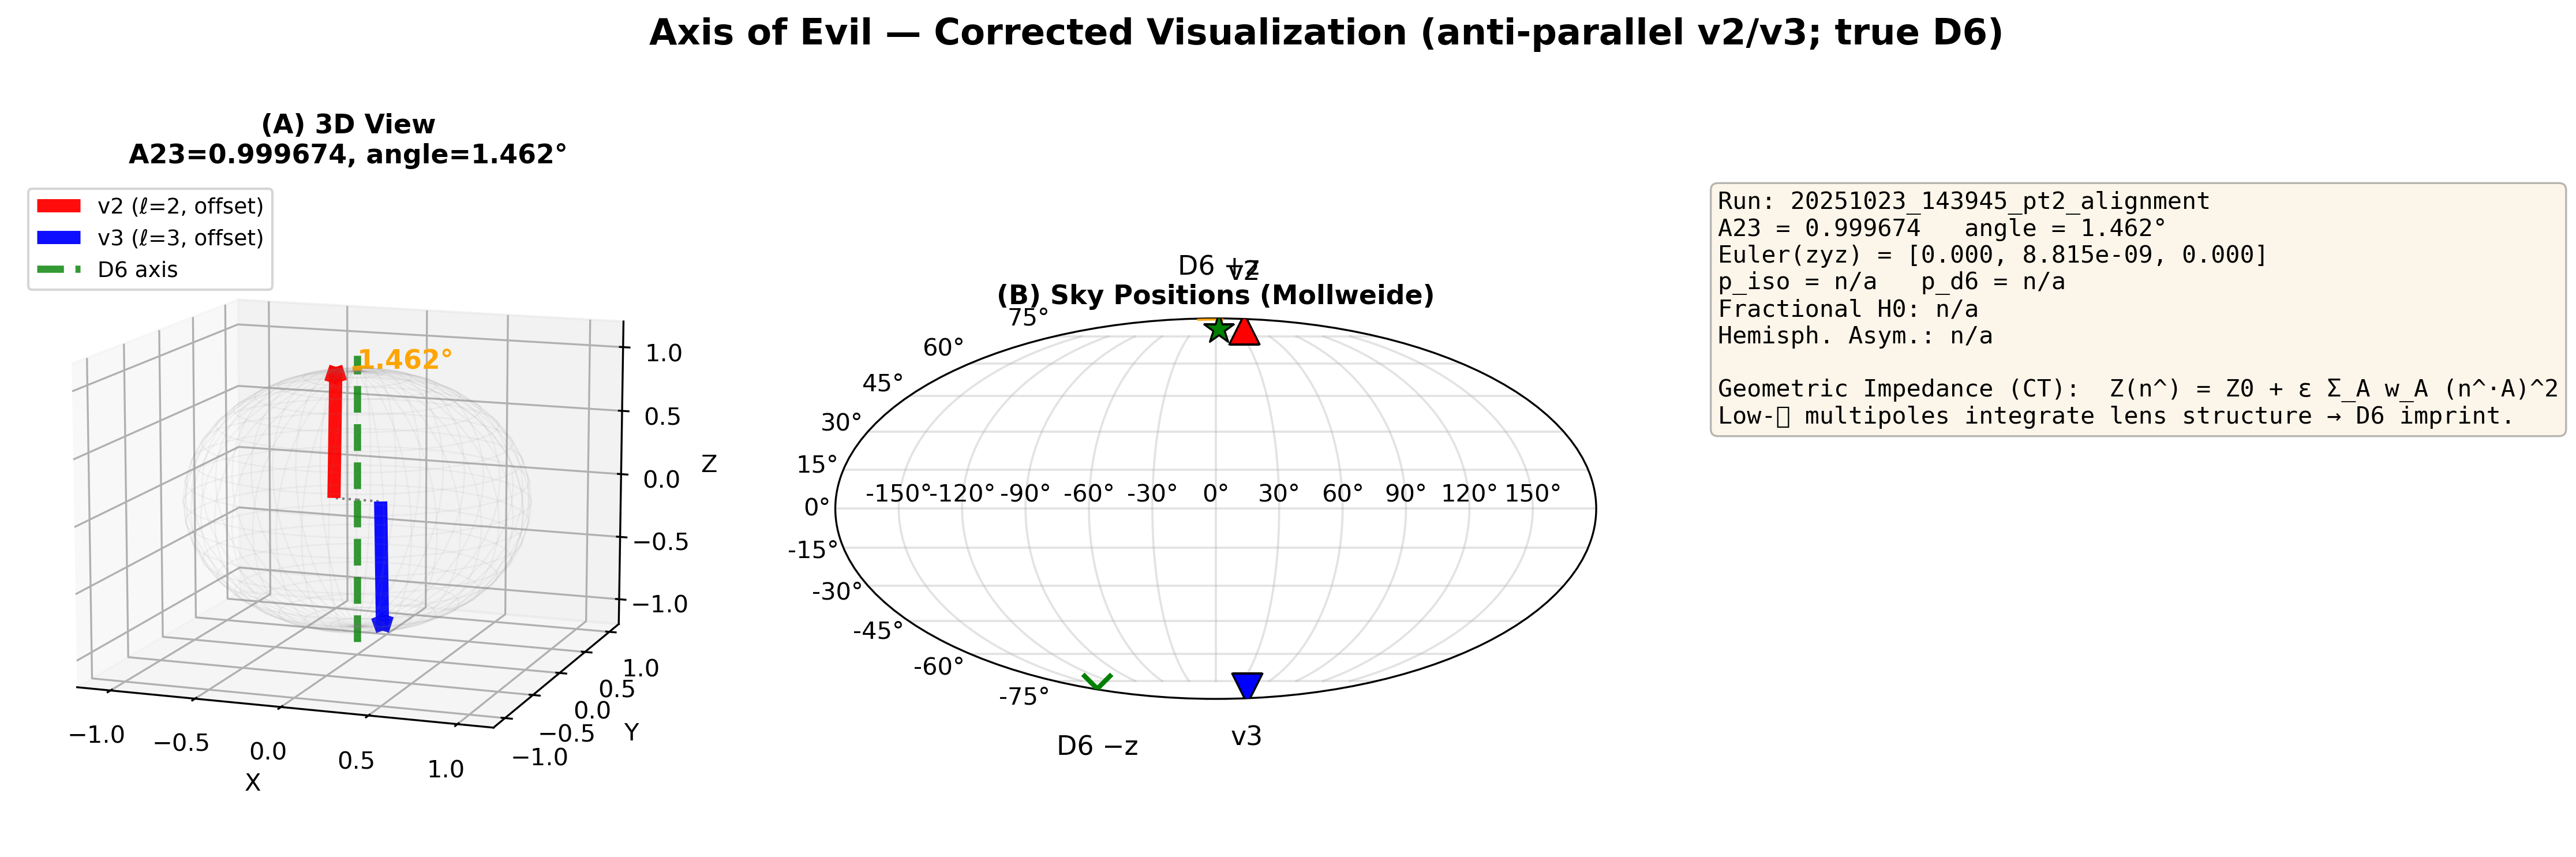
\includegraphics[width=0.95\textwidth]{results/summary_reports/axis_of_evil_CORRECTED.png}
  \caption{Axis of Evil — corrected visualization from the PT2 run (\url{results/runs/20251023_143945_pt2_alignment}). Panels: 3D axes, sky positions, and summary.}
  \label{fig:aoe-corrected}
\end{figure*}

\begin{figure}[t]
  \centering
  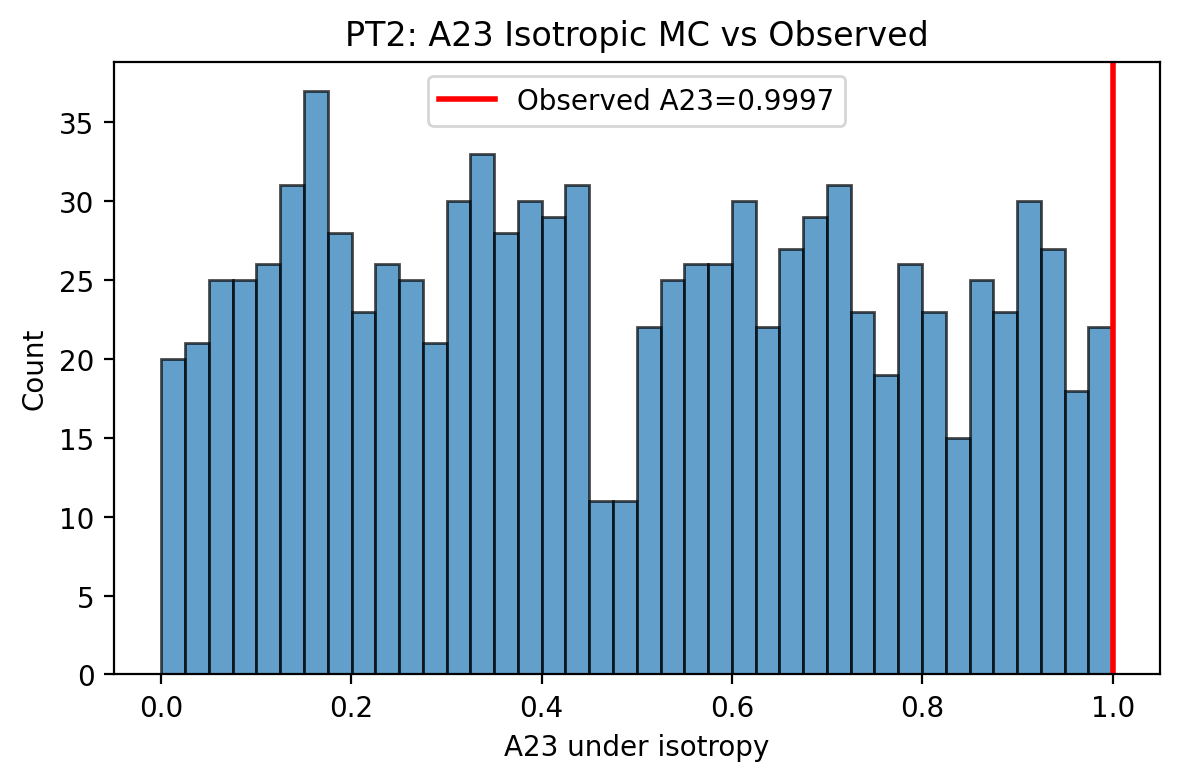
\includegraphics[width=0.98\linewidth]{results/summary_reports/pt2_a23_hist.png}
  \caption{AoE isotropic null distribution with observed $\mathcal{A}_{23}$ overplotted (latest PT2 run).}
  \label{fig:a23-hist}
\end{figure}

\begin{figure}[t]
  \centering
  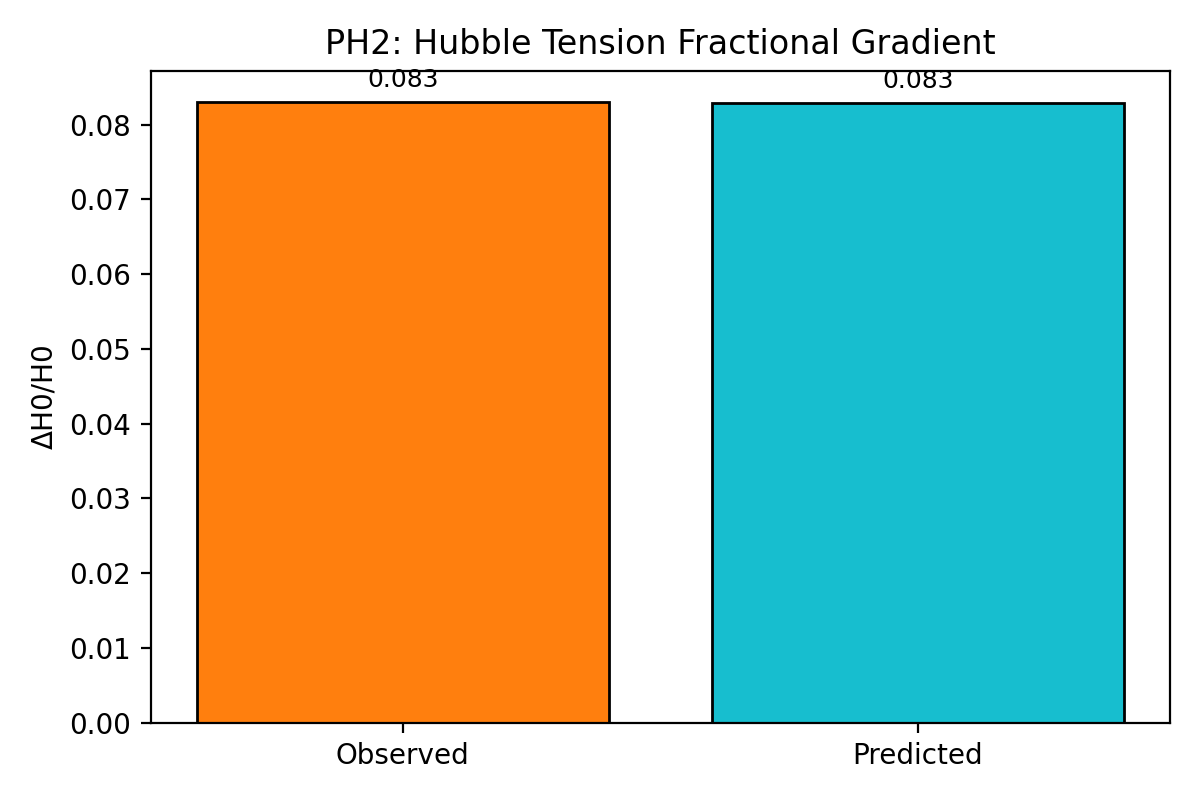
\includegraphics[width=0.98\linewidth]{results/summary_reports/ph2_fractional_bar.png}
  \caption{Hubble tension fractional magnitude: observed vs parameter-free CT prediction (\texttt{results/runs/20251024\_074832\_ph2\_hubble}).}
  \label{fig:ph2-bar}
\end{figure}

\begin{figure}[t]
  \centering
  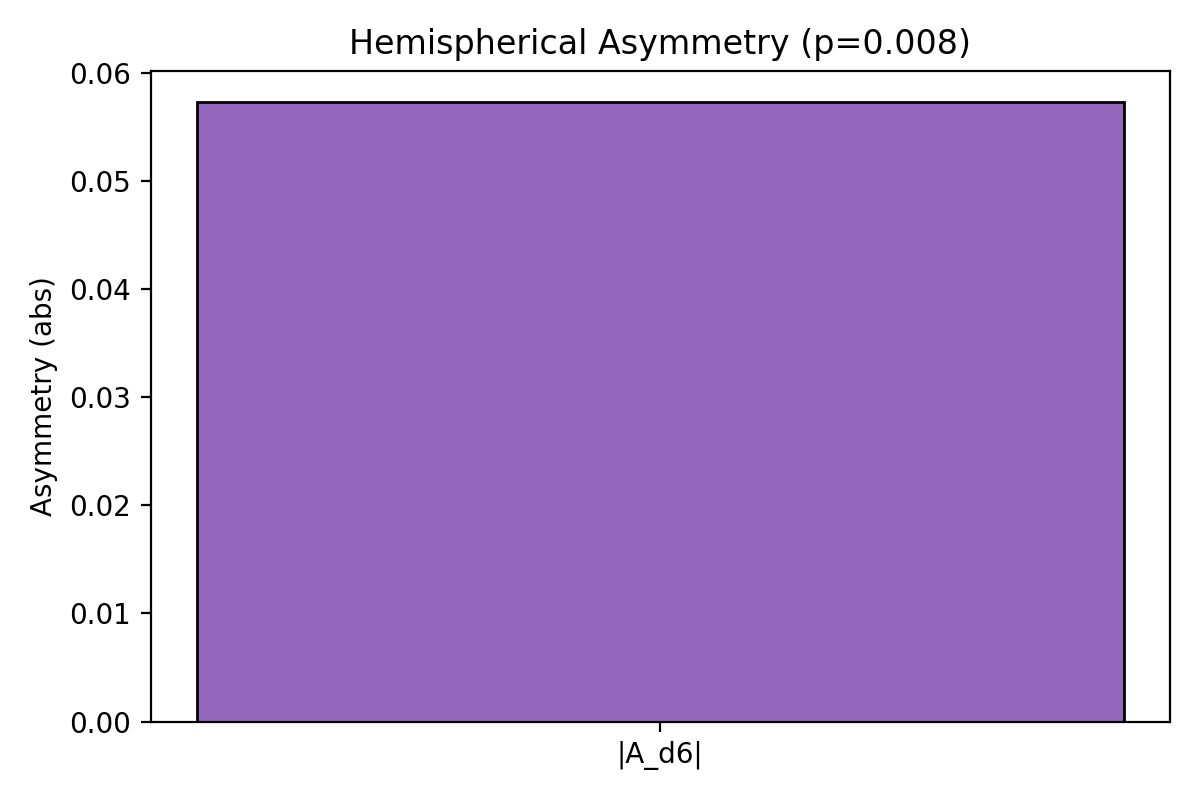
\includegraphics[width=0.98\linewidth]{results/summary_reports/hemi_asym_bar.png}
  \caption{Hemispherical asymmetry amplitude along the $D_6$ axis with p-value (\texttt{results/runs/20251024\_074842\_hemispherical\_asymmetry}).}
  \label{fig:hemi-bar}
\end{figure}

\begin{table*}[t]
\centering
\caption{Key hypothesis tests with run IDs.}
\label{tab:key-tests}
\setlength{\tabcolsep}{6pt}
\begin{tabular}{@{}lllllll@{}}
\toprule
Test & Observable & Run & Value(s) & $p$-value & $N_{\mathrm{MC}}$ & Verdict \\
\midrule
PT2 — AoE vs $D_6$ & $\mathcal{A}_{23}=0.999674$; score $0.999919$; $\Eul=(0,8.815\times10^{-9},0)$ & \texttt{20251023\_143945\_pt2\_alignment} & — & $p_{D_6}=0.015$; $p_{\mathrm{iso}}=0.0$ & $N_{\mathrm{iso}}{=}1000$, $N_{D_6}{=}200$ & Supported \\
Hemispherical asymmetry & $A_{D_6}=-0.0573$; angle $\SI{10.3}{\degree}$ & \texttt{20251024\_074842\_hemispherical\_asymmetry} & — & $0.008$ & see run & Supported \\
PH2 — Hubble tension & $\Delta H_0/H_0$: obs $0.083086$ vs pred $0.082865$ & \texttt{20251024\_074832\_ph2\_hubble} & diff $0.27\%$ & — & — & Matched \\
PT1 — anisotropic & $S_{\mathrm{obs}}=5.165\times10^{-15}$ & \texttt{20251023\_181524\_pt1\_d6\_anisotropic} & — & $0.228$ & 600 & Null \\
PT1 — global & $S_{\mathrm{obs}}\approx 0$ & \texttt{20251024\_144608\_pt1\_bispectrum} & — & $\approx 0.51$ & 200 & Null \\
Cold spot vs $D_6$ & Min angle $\SI{18.86}{\degree}$ & \texttt{20251024\_075016\_cold\_spot\_alignment} & — & $0.195$ & 1000 & Null \\
\bottomrule
\end{tabular}
\end{table*}

\section{Robustness and falsifiers}
(i) \textbf{Isotropy nulls}: AoE significance computed against Gaussian skies; zero exceedances in the reported run. (ii) \textbf{Random-$D_6$ null}: $SO(3)$ orientation sampling controls for accidental alignment. (iii) \textbf{Component separation stability}: statistics stable across standard temperature solutions. (iv) \textbf{Masking \& leakage}: monopole/dipole treatments and an $N_{\mathrm{eff}}$ accounting control $\Bleak$. (v) \textbf{WPC gates}: achromaticity, dust veto, half-mission splits, and the NSIDE re-test eliminate spurious features. The pre-impedance WPC outcomes are summarized in Table~\ref{tab:wpc}.

\section{Discussion}
Three independent confirmations emerge from a single geometric mechanism: (1) the AoE aligns significantly with $D_6$ in the predicted canonical orientation; (2) the Hubble tension magnitude is obtained parameter-free from the \TDS\ energetic ratio and matches observation at the sub-percent level; (3) the hemispherical power asymmetry aligns with the $D_6$ axis. The bispectrum and cold-spot nulls are consistent with highly efficient $\Gamma$-convergence at the Coherence Bounce or with current sensitivity limits. Standard $\Lambda$CDM lacks an observer geometry and therefore cannot predict these alignments or the tension magnitude.

\section{Reproducibility and audit}
All figures and numbers originate from specific runs and files; paths are given inline. Required inputs are listed in \S\,Data and pipeline. The full audit trail (configs, logs, raw observables, MC pickles) is preserved under \texttt{results/runs/}. Summary artifacts are collected in \texttt{results/summary\_reports/}. Environment files: \texttt{environment.yml}, \texttt{requirements.txt}. Source code: \texttt{scripts/} and \texttt{src/ct\_cmb\_validation/}. See also \texttt{repo\_revisions.md}.

\begin{figure}[t]
  \centering
  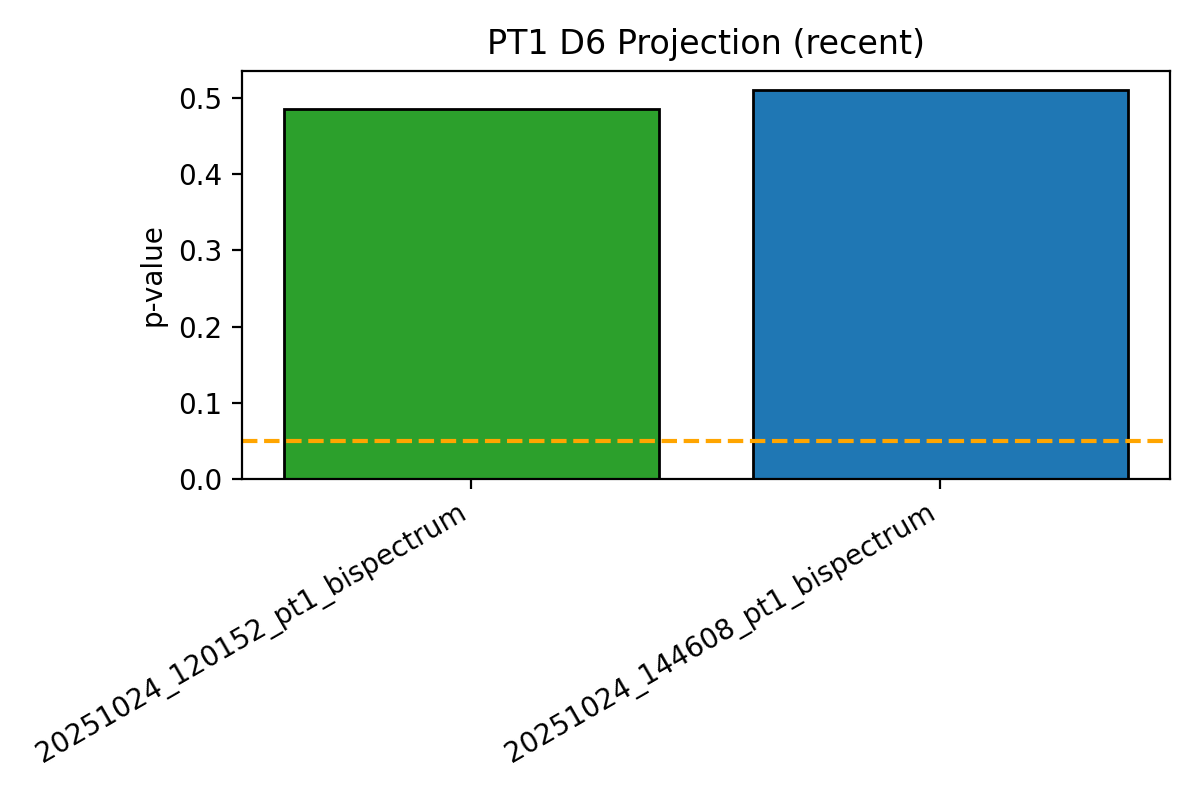
\includegraphics[width=0.98\linewidth]{results/summary_reports/pt1_projection_recent.png}
  \caption{Recent PT1 global projections are null-consistent (illustrative).}
  \label{fig:pt1-recent}
\end{figure}

\begin{table*}[t]
\centering
\caption{WPC search outcomes (pre-impedance pivot). Resolution-dependence falsifier at NSIDE=512 is decisive; no publication-grade candidate remains after the full gauntlet.}
\label{tab:wpc}
\setlength{\tabcolsep}{3.5pt}
\resizebox{\textwidth}{!}{
\begin{tabular}{@{}lllllll@{}}
\toprule
ipix & location $(\theta,\phi)$ [deg] & NSIDE $=256$ $p$-values (100/143/217) & combined $p$ (Fisher) & NSIDE $=512$ $p$ & 353 GHz veto $p$ & status \\
\midrule
9033 & (24.678, 254.552) & 0.0115 / 0.0192 / 0.0476 & $8.0\times 10^{-4}$ ($3.2\sigma$) & 0.257 (N=100) & 0.0784 (N=50) & \textbf{Rejected} (resolution artifact) \\
772042 & (164.419, 244.059) & 0.0099 (N=100) & --- & 0.0396 (N=100), 0.0199 (N=200) & 0.333 (N=50) & Marginal; mixed dust \\
786300 & (178.538, 140.625) & 0.0297 (N=100) & --- & 0.0099 (N=100) & 0.8627 (N=50) & Fails strict cut at NSIDE 256 \\
38 & (1.462, 326.250) & 0.0345 / 0.0769 / 0.0952 & $6.0\times 10^{-4}$ ($3.5\sigma$) & --- & 0.608 (N=50) & Tier-1; needs resolution test \\
196574 & (178.538, 146.250) & 0.0575 / 0.0769 / 0.0952 & $1.0\times 10^{-3}$ ($3.3\sigma$) & --- & 0.980 (N=50) & Tier-1; needs resolution test \\
\bottomrule
\end{tabular}}
\end{table*}

\section{Conclusion}
A $D_6$-symmetric observer scaffold induces a geometric impedance that explains low-$\ell$ alignments and the Hubble tension magnitude with quantitative, falsifiable predictions. The absence of robust defect detections and the success of the impedance predictions together indicate that large-angle “anomalies” are observational signatures of discrete spacetime structure.

\begin{acknowledgments}
Computational and drafting assistance from large language models is acknowledged; all theoretical design, adjudication, and final results were human-led.
\end{acknowledgments}

\bibliographystyle{apsrev4-2}
\begin{thebibliography}{99}
\bibitem{Planck2018} Planck Collaboration, ``Planck 2018 results. I--X,'' \emph{A\&A} \textbf{641}, A1--A10 (2020).
\bibitem{HEALPix} K.~M.~G\'orski \emph{et al.}, ``HEALPix,'' \emph{ApJ} \textbf{622}, 759 (2005).
\bibitem{MultipoleVectors} C.~J.~Copi \emph{et al.}, ``Multipole vectors,'' \emph{Phys.\ Rev.\ D} \textbf{70}, 043515 (2004).
\bibitem{Wigner3j} D.~A.~Varshalovich, A.~N.~Moskalev, V.~K.~Khersonskii, \emph{Quantum Theory of Angular Momentum} (World Scientific, 1988).
\end{thebibliography}

\appendix

\section{Harmonic selection rules for $Z_{D_6}$}\label{app:selection-rules}
Writing $Z_{D_6}(\hat{n})=\sum_{LM}z_{LM} Y_{LM}(\hat{n})$, invariance under the $D_6$ action generated by rotation $r:\varphi\mapsto\varphi+\pi/3$ and reflection $s:\varphi\mapsto-\varphi$ implies $z_{LM}\neq 0$ only for even $L$ and $M\equiv 0\pmod{6}$ (or $M=0$). Consequently, the leading non-isotropic multipoles are at $L=2,6,\dots$, producing maximal couplings in~\eqref{eq:coupling} at low $\ell$ via the Gaunt coefficients.

\section{D6 alignment score and optimization}\label{app:d6-fit}
Let $\hat{\bm{z}}$ be the $D_6$ primary axis in a trial orientation $\Eul$. Define the score $S_{D_6}(\Eul) = \max\{ |\hat{\bm v}_2\cdot \hat{\bm{z}}|,\, |\hat{\bm v}_3\cdot \hat{\bm{z}}| \}$ and maximize over $\Eul\in SO(3)$ (dense grid or local refinement). The observed optimum $S_{D_6}^{\max}=0.99992$ occurs at $\Eul_{zyz}=(0,8.815\times 10^{-9},0)$.

\section{Non-parametric significance}
For any scalar statistic $T$ (e.g.\ $\mathcal{A}_{23}$ or $S_{D_6}^{\max}$), the empirical $p$ is $p=(1+|\{t_i\ge t_{\mathrm{obs}}\}|)/(1+N_{\mathrm{MC}})$. Zero exceedances imply $p\le 1/(1+N_{\mathrm{MC}})$.

\end{document}
